\documentclass{article}
\usepackage[utf8]{inputenc}
\usepackage{tikz}
\usetikzlibrary{automata,positioning}
\begin{document}

\section{Introduction}

In Zebradb the concept of variable domain is the set of all possible values a variable can have,
for example, given the following zebradb definitions:

\begin{itemize}
      \item (number 0)
      \item (number 1)
      \item \ldots
      \item (number 9)
      \item and the query ?(number $'v$)
\end{itemize}

The query will unfy with all (number 0) \ldots (number 9) definitions and therefor $'v \in [0 \ldots 9]$ which is $'v$ domain.

\section{Why Zebradb needs them (The Problem)}

When zebradb search for query solutions, it unifies query tuples with definitions, for each unification it creates a branch that 
will contain unification changes.

Using the previews example, the query ?(number $'v$) will create 10 branches:

\begin{itemize}
      \item (number 0) unify (number $'v$) = (number 0)  
      \item (number 1) unify (number $'v$) = (number 1)
      \item \ldots
      \item (number 9) unify (number $'v$) = (number 1)
\end{itemize}

This is a simple query, the problem is when we start to have queries with more variables, even a simple definition like 
((number 'x) (number 'y)) will create 100 branches to solve the query ?((number 'x) (number 'y)).

The exponential growth of branches its a critical problem that needs to be solved to make zebradb useful.

To solve this problem we are still using branches for each unification, because this enables unification to run in 
parallel, but after each tuple unification we calculate variable domains, reducing the number of branches. 

For example, the query ?((number 'x) (number 'y)) can be solved has $'x \in [0 \ldots 9]$ and $'y \in [0 \ldots 9]$
dramatically reducing the number of branches needed for next iteration.


\section{The Solution}

As state on this post the solution I am investigating is the construction of variable domains, however 
this is not as simple has extracting values, because we need to consider two complications:

\begin{enumerate}
\item Deferred variables, a variable domain should not contain other variable,
\item Variable dependencies, variable domains are affected by other variables values.
\end{enumerate}

For example, the NAND operator can be defined as:

\begin{enumerate}
\item (0 nand 0 = 1)
\item (0 nand 1 = 1)
\item (1 nand 0 = 1)
\item (1 nand 1 = 0)
\end{enumerate}

Now consider the query ?('p nand 'q = 'r)

\begin{enumerate}
\item If  p=0 and 'r=1 then $'q \in [0, 1]$
\item If 'q=0 and 'r=1 then $'p \in [0, 1]$
\item Else 'p=1 and 'q=1 and 'r=0
\end{enumerate}

This gives us 3 branches, sometimes we don't win much or nothing using domains, in this case 3 is better then 4.

So I am working on an algorithm to extract domains, using automaton minimization, I will explain it with other 
example.

Consider the following definitions:
\begin{enumerate}
\item (mary likes food ')
\item (mary likes wine ') # likes(mary,wine).
\item (john likes wine ') # likes(john,wine).
\item (john likes mary ') # likes(john,mary).
\item (peter likes peter ') # likes(peter,peter).
\item (john likes 'stuff (mary likes 'stuff ')) # 1. John likes anything that Mary likes
\item (john likes 'person ('person likes wine ')) # 2. John likes anyone who likes wine
\end{enumerate}

And the query: ?(john likes 'stuff 'p)

First we extract query variables ['stuff, 'p], and then we construct a finite automaton using 
values extracted from branches generated by unifying the query with definitions,

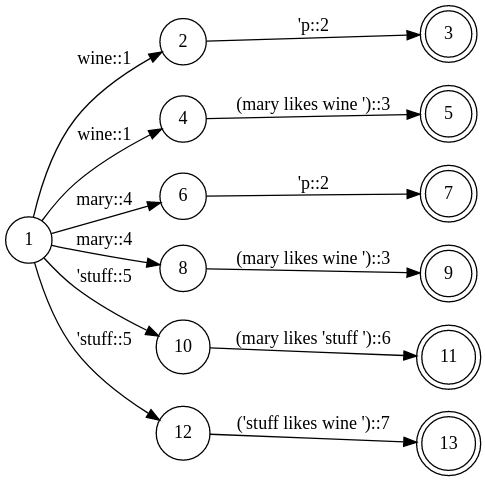
\includegraphics{sources/posts/variables domain (part 1)/john_likes_nfa.png}

The first level of values on the automaton corresponds to the first variable 'stuff and the 
second level to variable 'p. Basically we are creating a automaton with other like this (variable, value).

And next I perform a minimization:

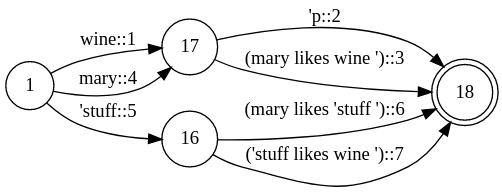
\includegraphics{sources/posts/variables domain (part 1)/john_likes_min.png}

And now I extract domains from minimized automaton, there is 2 rules for extraction:

\begin{enumerate}
\item There is a domain for each to state,
\item Domains can't contain variables and values at same time, so if we find a variable we split domain.
\end{enumerate}

So in this example to extract domain do the following steps:

\begin{enumerate}
\item We start from state 1 (start state),
\item Extract domain from state 1 to 17, stuff = [wine, mary],
\item Extract domain from state 17 to 18, p = ['p, (mary likes wine ')],
\item So the resulting domain is \{stuff: [wine, mary], p: ['p, (mary likes wine ')]\},
\item Since p contains a variable we need to split domain: [
      \{stuff: [wine, mary], p: ['p]\},
      \{stuff: [wine, mary], p: [(mary likes wine ')]\}
],
\item From start to state 16, extract domain: stuff = ['stuff],
\item From 16 to 18 extract domain: p = [(mary likes 'stuff), ('stuff likes wine)],
\item resulting domain is: \{stuff: ['stuff], p: [(mary likes 'stuff), ('stuff likes wine)]\}
\end{enumerate}

And finally we get the list of possible domains:
[
      \{stuff: [wine, mary], p: ['p]\},
      \{stuff: [wine, mary], p: [(mary likes wine ')]\},
      \{stuff: ['stuff], p: [(mary likes 'stuff), ('stuff likes wine)]\}
]

After having the domains, we create branches changing variables to domains or 
to values/variables (case domain is length 1)

The final result is like this: 

\begin{enumerate}
\item ?(john likes 'stuff 'p): 
      \begin{enumerate}
      \item @(john likes 'stuff {{v\$83 : ('stuff likes wine '\$1) (mary likes 'stuff ')}});
      \item @(john likes {{v\$80 : mary wine}} 'p);
      \item @(john likes {{v\$80 : mary wine}} @(mary likes wine '))
      \end{enumerate}
\end{enumerate}

And thats it, if we try to expand domains we get:

\begin{enumerate}
\item ?(john likes 'stuff 'p): 
      \begin{enumerate}
      \item @(john likes 'stuff ('stuff likes wine '\$1));
      \item @(john likes 'stuff (mary likes 'stuff '));
      \item @(john likes mary 'p);
      \item @(john likes wine 'p);
      \item @(john likes mary @(mary likes wine '))
      \item @(john likes wine @(mary likes wine '))
      \end{enumerate}
\end{enumerate}

So we actually got a pretty good compression, representing 6 branches with only 3 branches.

The next step is to handle tuples on the rest of processing pipeline, thats why the first two items 
of expanded tuples are an incomplete solution. 

Thats it.

\end{document}